\subsection{Werkzeuge}

\subsubsection{Robot Operating System (ROS)}

Das Robot Operating System ist ein frei verfügbares Framework zur Entwicklung von Roboter-Anwendungen. Die Verwaltung einer Vielzahl von Treibern, Bibliotheken und Tools vereinfacht die Arbeit an Robotern. Durch den Einsatz von Tutorials und Beispielen wird der Einstieg in die Entwicklung mit ROS sehr erleichtert. Die Kommunikation der entwickelten Programme, die sogenannten Nodes, erfolgt über Topics. Wie in Abbildung \ref{fig:ROS_concepts} schematisch dargestellt ist, werden die Daten, die von einer Node
ausgegeben werden sollen mit einem Titel, dem Topic, versehen und einem Pool an Topics hinzugefügt.

\begin{figure}[h!]
 \centering
		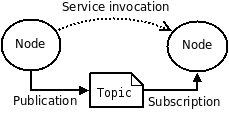
\includegraphics[width=0.4\textwidth]{drive/ROS_concepts.png}
	\caption{ROS Nachrichtenkonzept}
	\label{fig:ROS_concepts}
\end{figure}

Falls diese Daten folgend von einer anderen Node benötigt werden, kann diese das Topic einfach abhören und bekommt ausschließlich die gewünschten Daten übermittelt. Mit Hilfe des Nachrichtensystems lässt sich der Ablauf und die Synchronisation von einzelnen Funktionen des Roboters übersichtlich und einfach gestalten. Die Verwaltung von Nodes in Packages erleichtert darüber hinaus die Wiederverwendbarkeit des Codes. Darüber hinaus bietet ROS mit "Rviz" ein praktisches Tool zur Visualisierung von Daten, wie z.B. Laserscans oder Odometriedaten. Das Tool ist in Abbildung \ref{fig:Rviz} dargestellt und zeigt den Footprint des Robots und die Daten des Laserscans in Bezug auf die Umgebungskarte.

\begin{figure}[h!]
 \centering
		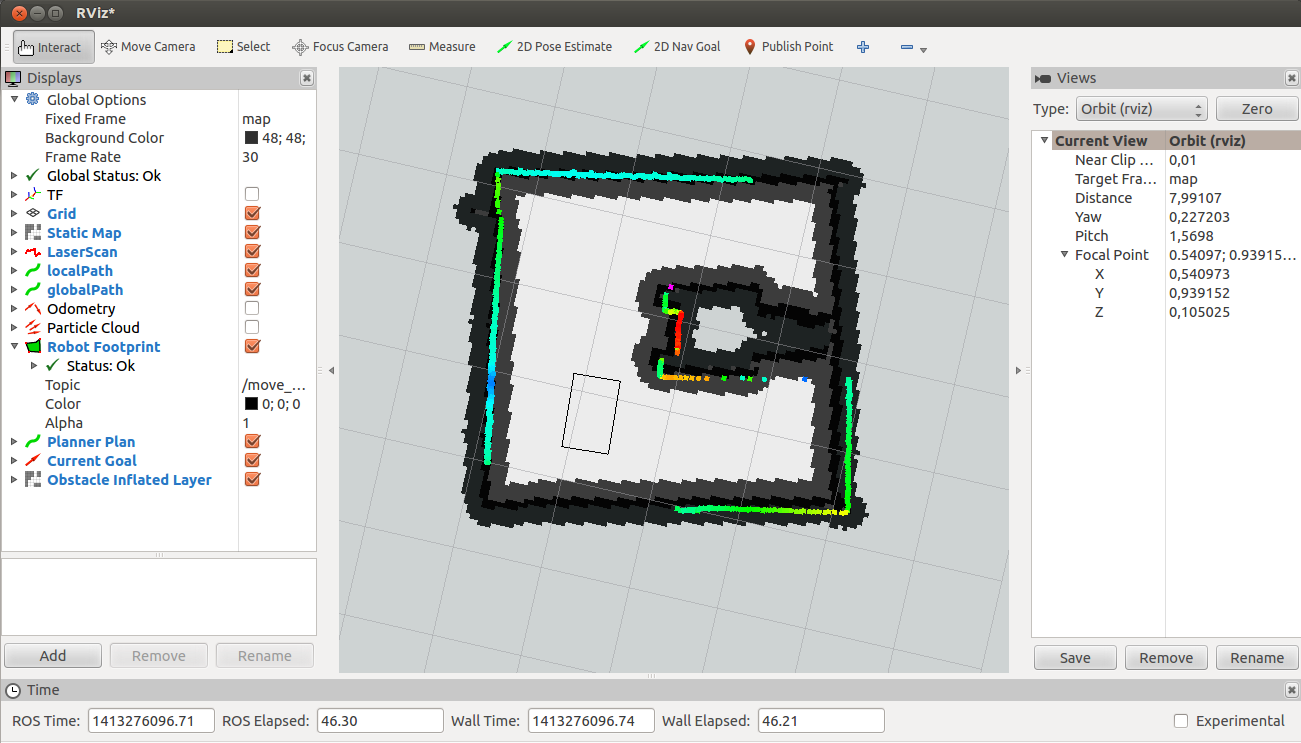
\includegraphics[width=1\textwidth]{drive/rviz.png}
	\caption{Das Visualisierungstool Rviz}
	\label{fig:Rviz}
\end{figure}

\newpage

\subsubsection{Epos Studio}

Das Epos Studio hilft bei der Verwaltung und der Steuerung der Epos-Controller. Es werden Funktionen bereitgestellt, mit denen es möglich ist die Controller anzusteuern oder auszulesen. Das Auslesen von Parametern der verschiedenen Epos-Controller unter Windows erleichterte die Initialisierung der Controller unter dem Ubuntu-Betriebssystems. Der Aufbau der Kommunikation wird im linken Abschnitt der Abbildung \ref{fig:Epos} dargestellt. Auf der rechten Seite der Abbildung befindet sich ein Tool zur Einstellung der Geschwindigkeit eines Epos-Controllers.

\begin{figure}[h!]
 \centering
		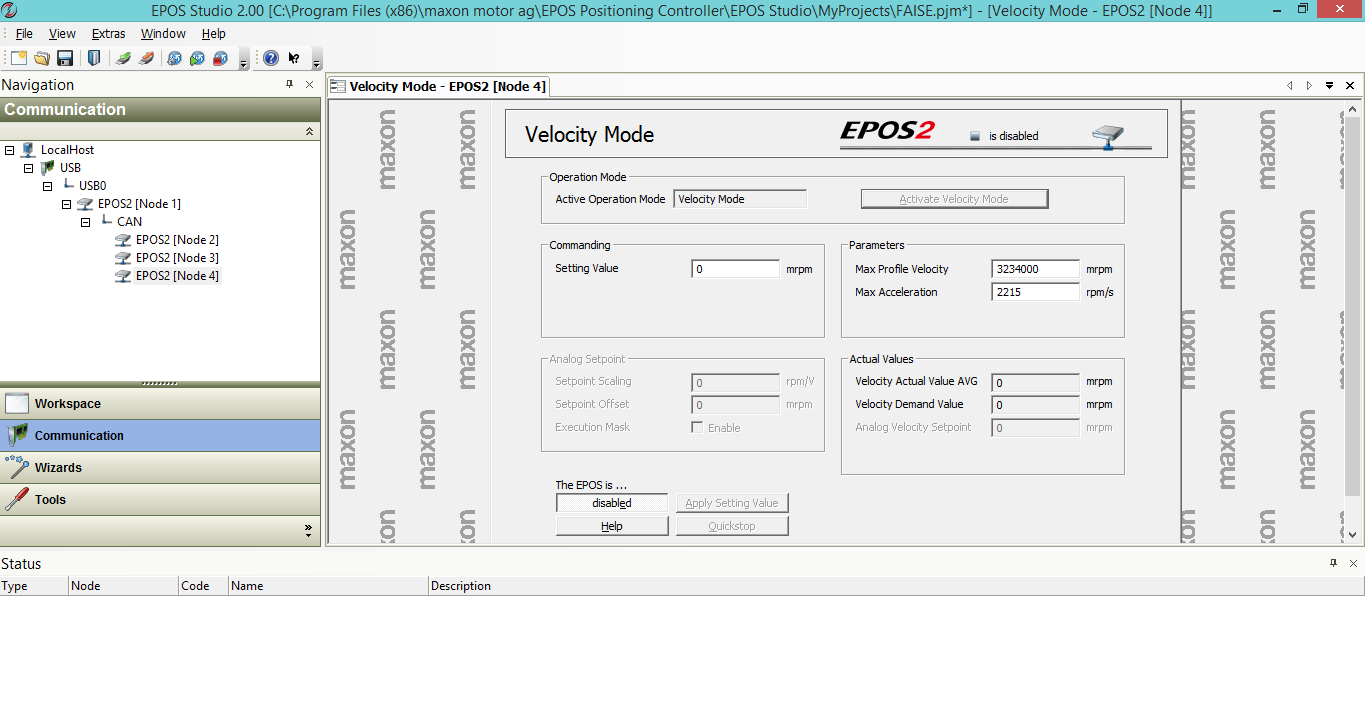
\includegraphics[width=0.9\textwidth]{drive/Epos_Studio.png}
	\caption{Das Epos Studio}
	\label{fig:Epos}
\end{figure}

\subsubsection{SOPAS Engineeringtool}

Bei SOPAS ET handelt es sich um ein Entwicklungsprogramm von Sick. Dieses wird zur Ansteuerung und Konfiguration der Laserscanner und Hallsensosren verwendet.

\begin{itemize}
\item \textbf{ Erster Start }

Beim ausführen von SOPAS wird ein neues Projekt erstellt, in dem man die gewünschte Hardware selektiert und einbindet. Die Wahl der Hardware erfolgt hierbei über den Netzwerkscanassistenten oder manuell über den Gerätekatalog. Sobald die Kommunikation mit der Hardware aktiv ist, kann diese angesteuert werden. Änderungen der Konfiguration der Hardware sind im Projektbaum möglich oder sogar notwendig ( siehe Kapitel 7.7 Herausforderungen).
\end{itemize}
